section{Literature Review Methodology}
\label{sec: methodology}

The methodology of the systematic review is mainly based on \cite{silva_systematic_2016} and complemented by \cite{moher_preferred_2009,thome_conducting_2016,durach_new_2017,snyder_literature_2019}. We structured our study according to the eleven steps presented in \cite{silva_systematic_2016}.

\subsection{Review Protocol}

This subsection serves as a review protocol, which should enable the reader to retrace the decisions that led to the final results \cite{moher_preferred_2009}. The presented protocol is the outcome of multiple iterations.

\subsubsection{Defining the main research questions of the literature review}

Based on the task to create a literature review on the state of research in data-driven inventory management, we developed three research questions, of which the answers reflect the current development of the research area:

\begin{itemize}
    \item RQ1: What do we know about the data quality of smartphone web surveys and what are current research gaps?
    \item RQ2: What do we know about survey design for smartphone web surveys and what are current research gaps?
\end{itemize}

\subsubsection{Defining keywords}
\label{subsubsec: Defining keywords}

After a first literature search and multiple iteration we identified the the following search string for our literature search:

\noindent (“mobile” OR “phone” OR “tablet” OR “device”) AND (“web” OR “online” OR “digital” OR “browser“) AND (“survey” OR “question*” OR “panel” OR “poll”) NOT ("bank*" OR "payment" OR “e-commerce” OR "health" OR "shop*" OR "library" OR "education" OR “sex*” OR “dating” OR “tourism” OR “travel” OR “social network” OR “social media” OR “internet of things” OR “iot” OR “advertis*”)

We identified this search string based on the precision and recall of the search terms combined with search settings (abstract search, title search, timespan, categories) for retrieving relevant entries. 


\subsubsection{Defining search engines}
\label{subsubsec: Defining search engines}

We selected the search databases based on the recommendations of the library of the University of Mannheim. We complemented the list with the publishers database of influential Journals of the research area. We excluded databases and articles where we had no free access as students of the University of Mannheim. The resulting final list comprised the following six databases:

\begin{itemize}
    \item  Web of Science
    \item ProQuest
    \begin{itemize}
        \item Applied Social Sciences Index \& Abstracts (ASSIA)
        \item Business Market Research Collection
        \item Sociological Abstracts
        \item Worldwide Political Science Abstracts
    \end{itemize}
    \item EBSCO
    \begin{itemize}
        \item APA PsycArticles
        \item APA PsycInfo
        \item PSYNDEX Literature with PSYNDEX Test
        \item Communication \& Mass Media Complete
    \end{itemize}
    \item Sage Journal
    \item Oxford Publisher
    \item Tanford Publishing
\end{itemize}

\subsubsection{Search string execution}

Based on the search string in \ref{subsubsec: Defining search string} we conducted the search in the databases mentioned in \ref{subsubsec: Defining search engines} on 20.12.2021. Additional setting that wer used when applicable in the search engines of the dabtaases are presented in Table \ref{tab: search settings}.The search was conducted searching in the Title, Abstract and Keywords if possible. If this was not possible we choose to search only the Abstract.

\begin{table}
	\caption{Additional settings for the search engines of the bibliographic databases}
	\centering
	\begin{tabular}{ll}
		\toprule
		Settings     & Values \\
		\midrule
		Time Horizon & Publications from year 2008 to 2021 \\ 
		Literature Type & Research Articles published in Proceedings and  Journals \\
		Journal Type & Peer-reviewed \\
		Research Field & Social Science, Political Science, Business /Economics, Computer Science, Psychology, Communication \\
		Language & English \\
		\bottomrule 
	\end{tabular}
	\label{tab: search settings}
\end{table} 

\subsubsection{Download and store search results}

The bibliographic details of the search results were downloaded as .ris files by offered download functions or scraped directly from the site with the bibliographic program Mendeley [citation]. The resulting files were all saved and managed in Mendely and Zotero. The search resulted in 2787 research papers and 1580 non duplicate entries.

\subsubsection{Define inclusion and exclusion criteria}

For the final selection of relevant articles for the literature review, we defined a set of inclusion and exclusion criteria. These criteria are the foundation to select relevant research articles in the selection stage.

\paragraph{Inclusion Criteria}
\begin{itemize}
    \item Research articles that focus on mobile web surveys
    \item Research articles that explicitly state the role of smartphones in mobile web surveys
    \item Research articles that are in English
    \item Research articles that were published between 2008 and 2021
    \item Research articles that are published in a peer-reviewed journal
    \item Research articles that are published in a peer-reviewed conference proceeding
\end{itemize}

\paragraph{Exclusion Criteria}
\begin{itemize}
    \item Research articles that do not differentiate the effects of different mobile devices like Tablet and Smartphone
    \item Research articles that use mobile devices only under supervision of an interviewer
    \item Research articles that just include mobile devices in web surveys without specifically analysing their impact
    \item Research articles on mobile forms in general
    \item Research articles focusing on mobile web tests or assessments
    \item Research articles about passive data collection with the smartphone
    \item Research articles that only focus on a small unrepresentative group in medical trials
    \item Research articles that present specific developed software
\end{itemize}

\subsubsection{Selection of papers - First and Second stage}

We screened the results of the literature search by title, abstract, and full text based on the mentioned inclusion and exclusion criteria. The title screening resulted in 147 articles, the abstract screening reduced it to 104 articles. We then found 12 additionall articles with a back and forward citaiton search. Resulting in 116 articles for the full tesxt search. After this step we had the final sample of 86 articles. Of which 12 were  were chosen as a result of a backward and forward citation search. The entire process of the selection of the paper can be seen in \ref{fig: Prisma Statement}.

\begin{figure}
    \centering
    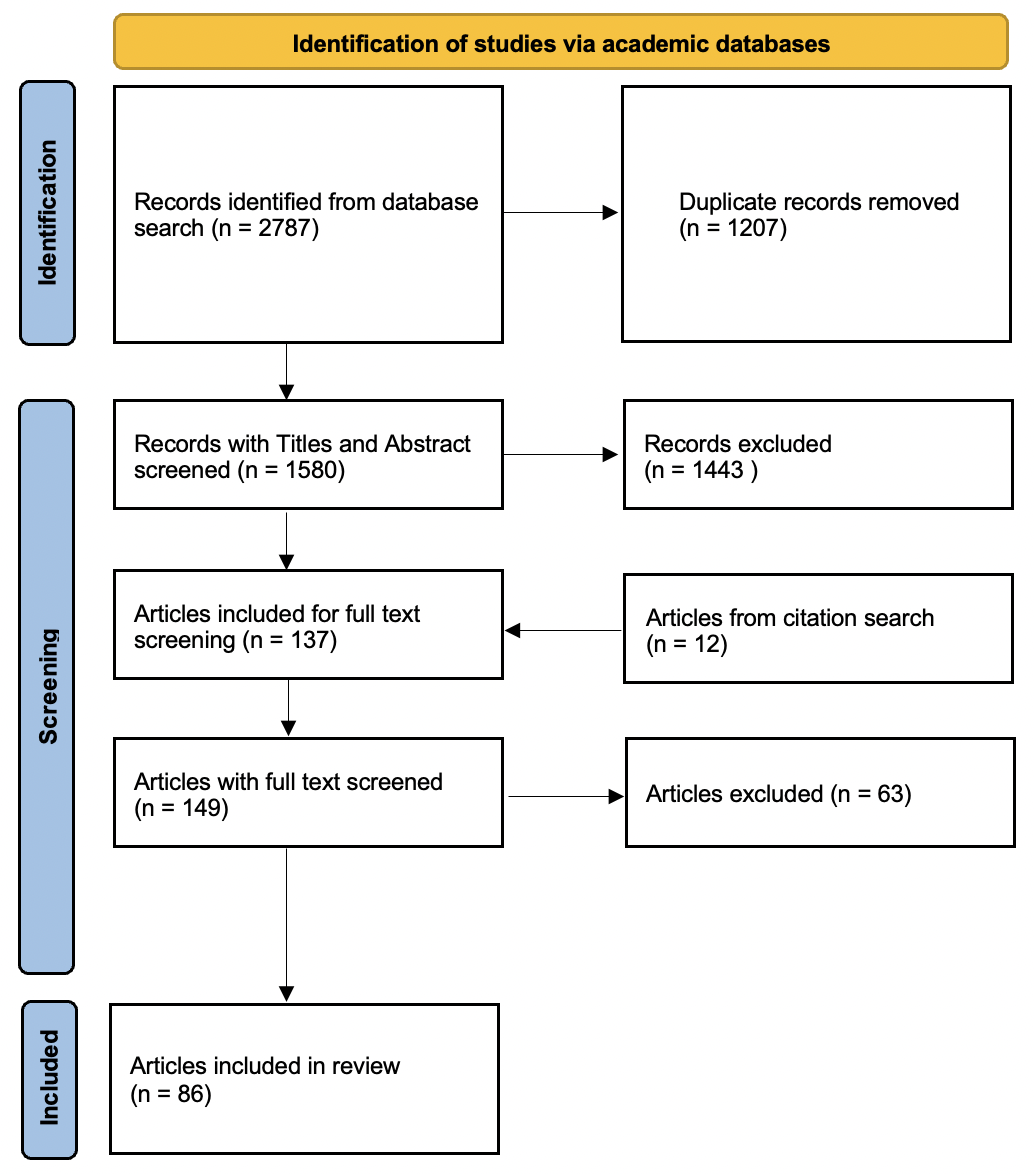
\includegraphics[width=\textwidth]{reports/figures/Prisma Statement.png}
    \caption{Prisma Statment for the systematic literature review in accordance with \cite{moher_preferred_2009} . doi: 10.1136/bmj.n71}
    \label{fig: Prisma Statement}
\end{figure}

\subsubsection{Extraction of answers related to research questions}

After the selection information for the analysis of the research question was extracted by a single coder. The information was saved in a spreadsheet, that was used for further analysis. We only retrieved results that were statistically investigated with a singificance level of 0.05. True if proofed by Logit Modelling oder Hypthesis test. Interested researcher can refer to the githup repo [citation] for an overview of the coded dimensions. The reader is referred to  \cite{langenbahn_data_2021} for all results of the information extraction. 


\subsection{Discussion of procedure}

Before analysing the results of the literature review we will critically discuss the procedure of the systematic literature review in this section. The presented work was done in the context of a postgraduate course work by a single student. We choose the guideline from \cite{silva_systematic_2016} and citation based on their feasibility for postgraduate students and the possibility to use the guidelines as a single reviewer. Other approaches like citations may be more appropriate for a more professional setup but were out of the scope of this coursework. However we still want to discuss the bias and weaknesses of this articleto to enable the reader to evaluate the objectivity of the presented results.


\subsubsection{Analysis of bias in this work}

To analyse for bias in this work we will base our analysis on \cite{durach_new_2017}. In this work there were multiple classes of bias identified which divide into sample bias, selection bias , within-study bias and expectancy bias. We will now analyse this work by the means of this dimensions.

The class of sample bias divides into retrieval and publication bias, that are both to a certain degree present in this work. Retrieval bias may occur in the selection of databases, the creation of the search strings and the search settings used. Our choice of databases was based on best practices promoted by the University of Mannheim libray but was limited to the resources available to students of the University of Mannheim, that excluded access to search engines like SCOPUS and some various articles that were hidden behind a paywall. This restriction will have lead with a high probability to a retrieval bias in this work. The search string and search setting showed a high recall with only 12 added articles from forward and backward citation search. As we included all important Journals and a high range of databases it is not probable that we have missed whole clusters of research articles, that we did not identify in the citaiton serach. The search string however has a very low precision, which has led to much ineffectual work, which has the potential induce mistakes in the selection. Another possibility for a retrieval and publication bias is that this review only used articles published in a peer reviewed scientific medium. Our citation search has showed that there a lot of impactful scientific works, taht are presented on conferences in a presentation fomrat [AAPOR, JASRO] or in editor reviewed Journal [Survey Practice]. Another work could include this grey literature in their review to get a more complete overview of the research field. 

Selection biases partition into inclusion and selector biases, where a selection bias is highly likely in this work and the selector biases rather insignificant. An inclusion bias implies nit adequately defined inclusion and exclusion criteria. This bias will be most likely be present in this work as no research experts for mobile web surveys designed the criteria. The selector bias is not significant through the setup with only one person creating inclusion and exclusion rules and selecting the articles, not having much space for inconsistencies.

The within-study bias describes errors in extracting information from the selected articles. AS only one person extracted information from the data, we cannot guarantee the quality of the extraction by measurement likes the inter-annotor agreement or similar. This has the potential to lead to within-study bias for this work.

The expectancy bias is the last category of biases, which is negligible in this work. The author of this work does not have any professional prior knowledge about mobile web surveys and do not have personal interest that could lead to any preconceptions.

\subsubsection{Future research}
In this section we wan to discuss how one could advance this review on the level of a scientific publication. We have already identified methodological weaknesses that need to be fixed in the last section. Additionally we will shortly discuss the range of topics in this work.  

To avoid technical mistakes, the replication of this work would need at least one experienced researcher with expertise in mobile web survey to use their domain knowledge and avoid the identified technical biases. Additionally another researcher is required to increase the robustness of the selection and information extraction. With more resources it would be possible to reduce the retrieval bias by including more search engines like Scorpus and gain access to paid articles. Further improvements could be the fine tuning of the search string and the inclusion of the characteristics of different search engines. To further avoid publication bias one could include qualified scientific literature not considered in this review. Another problem of this literature review as discussed in the next section was the breadth of the article, that lead to a missing depth in the analysis of the different topics. In a next research project one could concentrate on one dimension of smartphone web surveys to get a more sophisticated research article.

To summarize we can state that the present work not wholly fulfil all scientific standards but can function as basis for a further research work.